\begin{frame}{Git Basics}{Add/Commit}
  \begin{itemize}
    \item \textbf{git add}: To add a new file or modified into the staging (index) area. It makes 
      the changes ready for commiting.
      \comm{git add FILE\_NAME}
      \comm{git add .} (adds all the changes current directory and sub-directories)
    \item \textbf{git commit}: To put the staged files into the (local) repo. Such changes can be tracked, i.e.,
      revert, log, etc.
      \comm{git commit -m "A proper message"}
  \end{itemize}
  \begin{figure}
    \begin{center}
    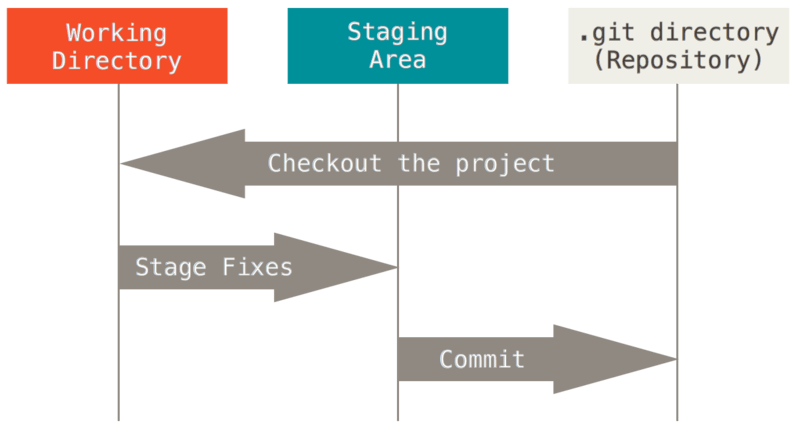
\includegraphics[width=0.55\linewidth]{pics/areas.png}
    \vspace{-0.3cm}
    \caption{\footnotesize Git areas (Source: https://git-scm.com)}
  \end{center}
\end{figure}
\end{frame}

\begin{frame}{Git Basics}{Initializing a repo}
  \begin{itemize}
    \item Creating a local repo (without any remote)
    \comm{git init} (creates .git sub-directory)
    \comm{echo "hello world." $>>$ firstFile.txt} (makes changes in  working area)
    \comm{git status} (You see that your commit has some hash value)
    \comm{git add firstFile.txt} (puts your changes into staging area)
    \comm{git status} (You see that your commit has some hash value)
    \comm{git commit -m "A proper message"} (Now you have your first commit on the default branch master)
    \begin{itemize}
      \item Hint:
      {\tiny {\color{blue}git commit -am "A proper message"} (combines "git add" and "git commit")}
    \end{itemize}
    \comm{git status} (A clean repo and one commit with a hash value)
    \comm{git branch -m master main} (renames the branch master to main)
    \comm{git remote} (Output is empty since there is no remote repo)
  \end{itemize}
\end{frame}


